\section{Arbejdsmetoder}
Af Kasper\\\\
En del af opgaven var at følge Scrum og Agile principper til at få fremstillet projektet. Gruppen tog dette nogenlunde til sig, dog krævede det en tilvænningsperiode i starten af samarbejdet før alle var med på hvordan dette skulle udføres.\\
Vi har været 4 mand i gruppen, og selvom Scrum bygger på grupper af 6-8 mand, har dette har været en meget passende størrelse i forhold til uddellegering af opgaver, og så er man ikke for mange til møderne, som derfor bliver overkommelig længde.
Derudover gør det mindre antal gruppemedlemmer også det, at det ofte er nemmere at komme til enighed i diskussioner, men at alles stemme bliver hørt, da hver mand jo tæller for 25\%.\\
Vi har i vores gruppe aftalt at vi de fleste dage mødtes på skolen for at arbejde, for at sikre os at alle får foretaget det de skal, og det på den måde bliver nemmere at hjælpe hinanden med problemer man måtte møde undervejs.

\subsection{Værktøjer}
Til versionsstyring har vi benyttet os af Git og GitHub. Dette har fungeret til al tilfredsstillelse, og vi har sjældent haft merge conflicts. Gruppen har sigtet efter at arbejde efter feature-branching, altså at hver ny tilføjelse laves i sin egen branch, og derefter merges ind i master til det fungerende projekt.\\\\
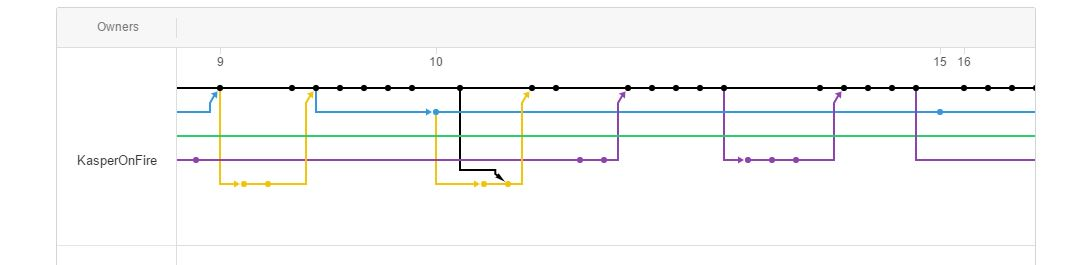
\includegraphics[width=\textwidth]{branches}\\\\


\subsection{Scrum}
Vi har arbejdet efter scrum i dette projekt. Dette har inkluderet daily standup meetings, sprint planning, sprint reviews og sprint retrospective meetings. Dette projekt har været god øvelse i at arbejde efter scrum's principper. Især daily standups har været effektive, da det hurtigt giver et overblik over hvad gruppen arbejdede med dagen før, og hvad der skal arbejdes med denne dag.

\subsection{Agile development}
Agile development kom nemt til gruppemedlemmerne som en teknik, da alle fokuserede på at levere funktionel kode og at være produktive individuelt. Enkelte gange har problemer krævet at 2 satte sig sammen og par-programmerede for at løse dette.